\section{Введение}
Фермент фруктозодифосфатальдолаза (EC=4.1.2.13) катализирует обратимое расщепление
фруктозо-1,6-дифосфата между С-3 и С-4 с образованием диоксиацетонфосфата и фосфатного эфира
изомерной альдотриозы (глицеральдегида). Равновесие сильно сдвинуто в направлении
обратной. Данная реакция является частью гликолиза. Также фермент участвует в гликонеогенезе и
было доказано, что иногда он может функционировать как адапторный белок.

Реакция образования глицеральдегид-3-Фосфата и дигидроксиацетонфосфата:\\
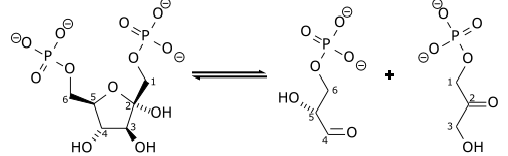
\includegraphics[width=0.8\linewidth]{intro-react}

В настоящее время фермент представляет собой тетрамер, состоящий из 4 одинаковых субъединиц (мол.
масса 162 kDa). Животные ткани содержат по меньшей мере три различные альдолазы, характерные для
мышцы, печени и мозга (A, B, C).

Пространственная структура альдолазы А из мышц кролика, рисунок был взят из банка данных PDB, код - 1ZAH:\\
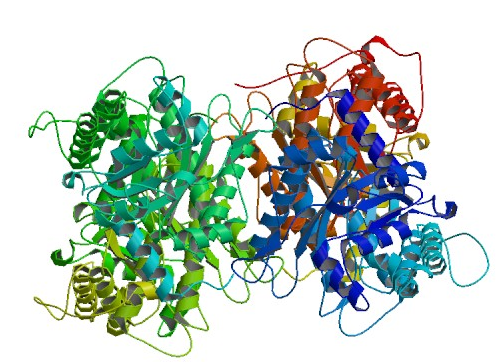
\includegraphics[width=0.8\linewidth]{intro-pdb}

A, B, C кодируются тремя разными генами и по-разному экспрессируются в течение развития организма.
Альдолазы А и С были найдены в взрослых тканях животных.
Кинетические параментры: для человека константа Михаэлиса Km=52 µM  для фруктозо-1,6-бисфосфата
(информация была взята с Uniprot, P00883 (ALDOA\_RABIT)).

